\documentclass[review]{elsarticle}

\usepackage{lineno,hyperref}
\modulolinenumbers[5]

\journal{Eugène Syriani, University of Montreal}

%%%%%%%%%%%%%%%%%%%%%%%
%% Elsevier bibliography styles
%%%%%%%%%%%%%%%%%%%%%%%
%% To change the style, put a % in front of the second line of the current style and
%% remove the % from the second line of the style you would like to use.
%%%%%%%%%%%%%%%%%%%%%%%

%% Numbered
%\bibliographystyle{model1-num-names}

%% Numbered without titles
%\bibliographystyle{model1a-num-names}

%% Harvard
%\bibliographystyle{model2-names.bst}\biboptions{authoryear}

%% Vancouver numbered
%\usepackage{numcompress}\bibliographystyle{model3-num-names}

%% Vancouver name/year
%\usepackage{numcompress}\bibliographystyle{model4-names}\biboptions{authoryear}

%% APA style
%\bibliographystyle{model5-names}\biboptions{authoryear}

%% AMA style
%\usepackage{numcompress}\bibliographystyle{model6-num-names}

%% `Elsevier LaTeX' style
\bibliographystyle{elsarticle-num}
%%%%%%%%%%%%%%%%%%%%%%%

\begin{document}

\begin{frontmatter}

\title{Visual Parametric Maze Generator DSL \tnoteref{mytitlenote}}
\tnotetext[mytitlenote]{Full source code is available on \href{https://github.com/Thealoe/ParametrizedMazeGen}{GitHub}.}

%% Group authors per affiliation:
\author{Corentin Moiny\fnref{myfootnote}}
\address{304, 5e Avenue Mailloux, La Pocatière. Quebec. Canada}
\fntext[myfootnote]{2020}

%% or include affiliations in footnotes:
\author[mymainaddress]{University of Montreal}
\ead{corentin.moiny@umontreal.ca}

\address[mymainaddress]{2900 Edouard Montpetit Blvd, Montreal, Quebec. Canada}

\begin{abstract}
(TODO) - This is a test abstract again and again.
\end{abstract}

\begin{keyword}
MDE \sep Maze \sep Generator \sep Parametric \sep Python \sep Epsilon \sep DSL \sep Java \sep Visual
\MSC[2010] 00-01\sep  99-00
\end{keyword}

\end{frontmatter}

\linenumbers

\section{Introduction}

\paragraph{A}
In the context of our Model-driven Engineering project assignment, I was charged to design a visual DSL to generate parametric mazes using a external Python program that I have also implemented. The goal of this project is to empower parameters understanding with the DSL and than produce probabilistic mazes. With this approach, anyone could generate maze with minimal or no engineering knowledge. Parametric maze generation is not a new concept, our approach was highly inspired by Design-Centric Maze Generation by Paul Hyunjin Kim and al\cite{kim_design-centric_2019}. From this paper I reused the maze cells concept where each one of them represent a 3x3 tiles on the maze. I also reused the same types of rates (and added one more), as in the paper, with a probabilist approach.

\paragraph{B}
(TODO) - Details of the sections presented

\section{Solution}

In this section, I give details on the solution choices used and the purposes behind theses.

\subsection{DSL}
The domain specific language represent the parameters used to generate the maze. Presented as a visual syntax in Figure \ref{fig:model}, it contains four types of generator. From left to right, generators are represented as blue rectangles: (1) \textit{RGen} is the first step of the maze generation, it gives the initial borders of the maze using a row count (\textit{RC}) and a column count (\textit{CC}) represented as red squares. (2) \textit{FPGen} inject maze cells in this initial shape to force a pattern, it allows users to create drawing in the maze. Cells are represented as orangish square (\textit{Marked 15 with a CP}) where a point is defined inside of it. In Figure \ref{fig:model}, we only force a single cell. (3) \textit{SPGen} is the generation of a solution path with specific parameters, allowing to gives different behaviours from the general maze body. Used rates are represented as green circles. (4) \textit{MBGen} is the last step, the maze body generation. Using rates as green circles also.

\begin{figure}
	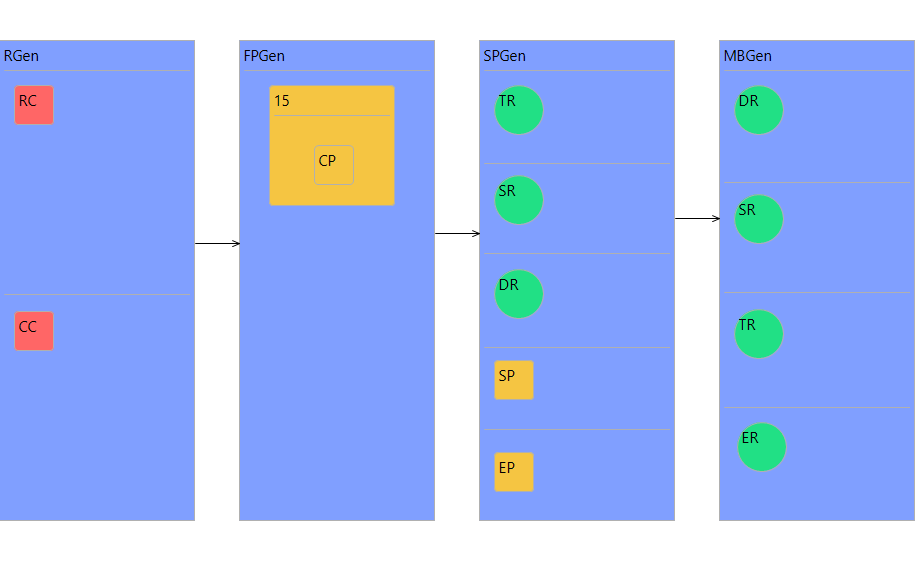
\includegraphics[width=\linewidth]{model.png}
	\caption{A model instance from the DSL}
	\label{fig:model}
\end{figure}

\paragraph{Types of rate}
The DSL uses 4 types of rates: (1) StraightRate marked as \textit{SR} that represent weight of straight path. (2) TurnRate marked as \textit{TR} that represent uni-directional turning path. (3) DecisionRate marked as \textit{DR} that represent bi-directional turns and crossroads. (4) EndRate marked as \textit{ER} that represent the famous dead-end, also known as  \textit{cul-de-sac}. Theses rate values will determine the behaviours of generation and will be used in a probabilist approach. A random number will be generated and is associated to a weighted value, it returns a list of cell types that represent this rate type. The list is than intersected with a possible neighbours list and a random cell is chosen as a type of cell.

\subsubsection{Meta-model}
As mentioned earlier, our DSL is a representation of different types of parameters to generate a maze. This generation a sequential order of four steps: rectangle, forced patterns, solution path, maze body.
-> Present root object, link with generators (4), shared rates, abstract classes, end rate...


\begin{figure}
	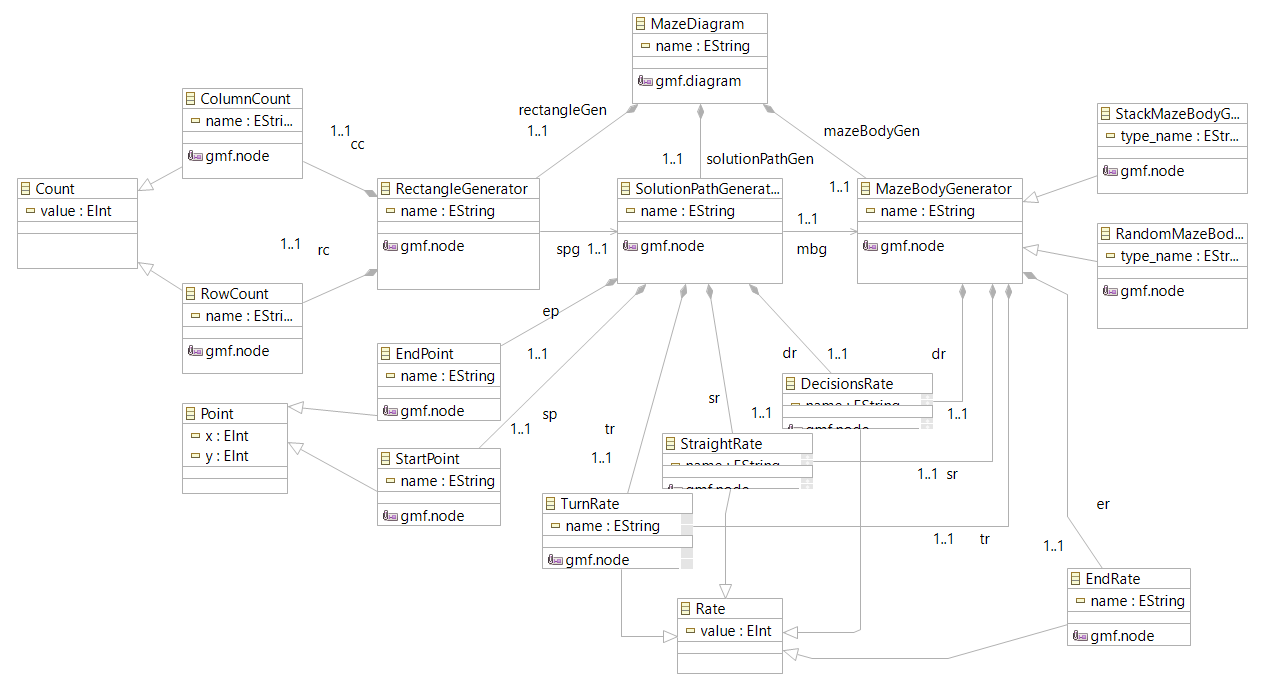
\includegraphics[width=\linewidth]{metamodel.png}
	\caption{Meta-model of the DSL}
	\label{fig:metamodel}
\end{figure}


\subsection{Generator}

\paragraph{Maze cells}
The generator uses a total of 16 maze cells types, as in Figure \ref{fig:cells}. Each cells have a list allowed neighbours, this list is computed in class \textit{AllowedCellTypeFeeder}. Generation algorithms will used this features to intersect will other desired cells types to make sure all cells can connect together at the end of the generation.

\begin{figure}
	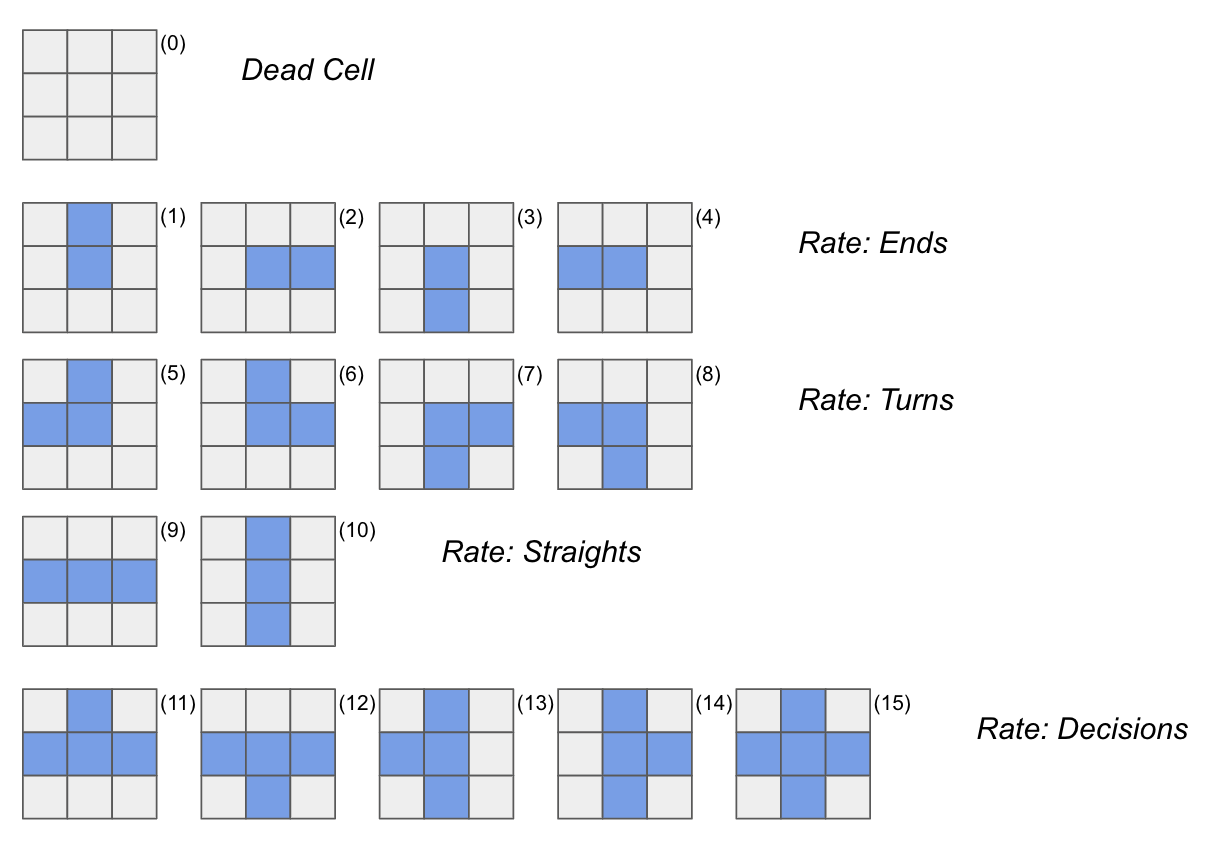
\includegraphics[width=\linewidth]{maze_cells_clean.png}
	\caption{Maze cells with associated rate type}
	\label{fig:cells}
\end{figure}

\section{Evaluation}

\section{Related Work}

\section{Conclusion}

\bibliography{mybibfile}

\end{document}